\section{Základní struktura na tranzistorové úrovni logických obvodů v bipolárních technologiích}
- AND, NAND, NOR, OR

   \begin{figure}[h]
   \begin{center}
     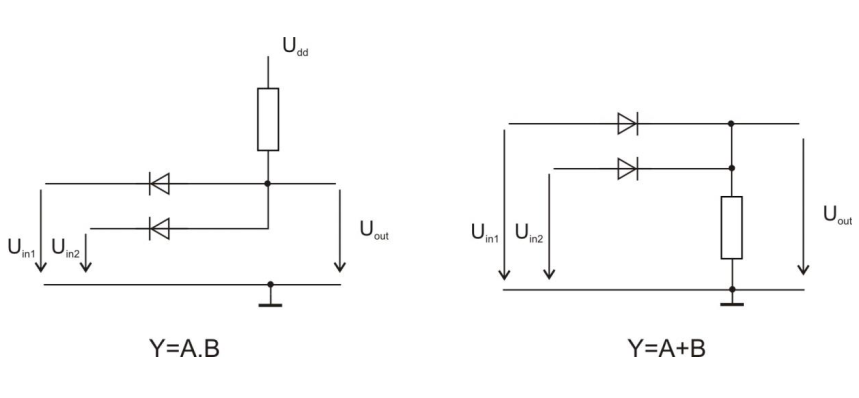
\includegraphics[scale=0.6]{images/dioda.png}
   \end{center}
   \caption{Realizace log. fce pomoci diod}
  \end{figure}
  
\subsection{NAND}
   \begin{figure}[h]
   \begin{center}
     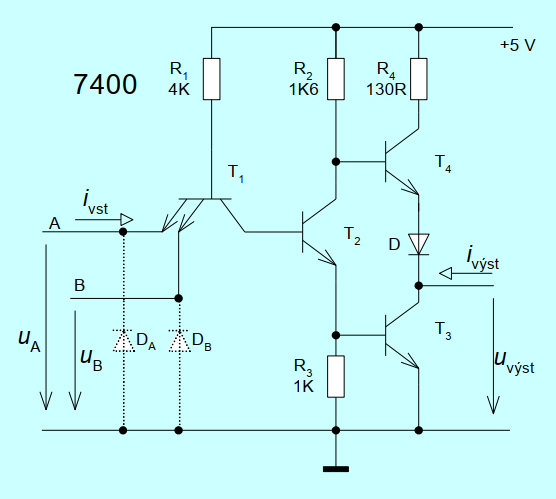
\includegraphics[scale=0.6]{images/NANDBJT.png}
   \end{center}
   \caption{Funkce NAND v BJT technologii}
  \end{figure}
  
  \subsection{NOR}
   \begin{figure}[h]
   \begin{center}
     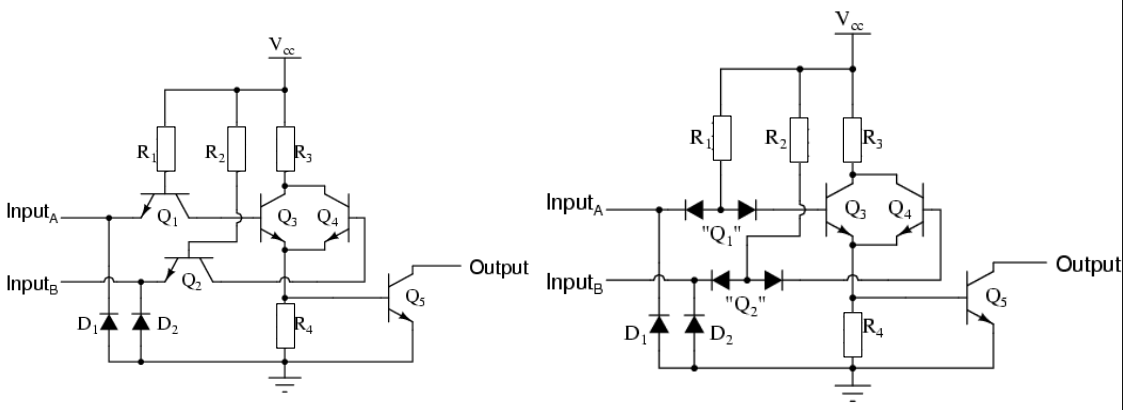
\includegraphics[scale=0.6]{images/NORBJT.png}
   \end{center}
   \caption{Funkce NOR v BJT technologii}
  \end{figure}
\pagebreak
\subsection{OR a AND}
Tyto obvody se skládají z NAND/NOR a poté je na jejich výstup zařazen invertor.
   \begin{figure}[h]
   \begin{center}
     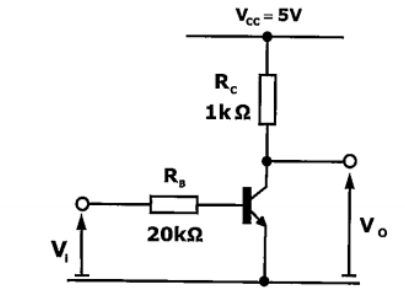
\includegraphics[scale=0.6]{images/INVBJT.png}
   \end{center}
   \caption{Funkce INV v BJT technologii}
  \end{figure}

